\section{2D Graphics}
2D Graphics primitives are procedures that draw simple geometric shapes based on a \textbf{2D coordinates system} , a set of integer with unit the \textbf{pixel} $ \to $ \textit{pixel coordinates}.\\
The coordinate system is \textbf{Cartesian} , with the origin on the \textbf{left-top} ranging from $$ 0 \leq x \leq s_w-1 $$ $$ 0 \leq y \leq s_h-1 $$
A \textbf{clipping} procedure avoids that coordinates go out of boundaries ,causing \textbf{wrap-arounds} or writing of \textbf{un-allocated memory space} 
\begin{figure}[!h]
\begin{minipage}{.5\textwidth}
 \centering
  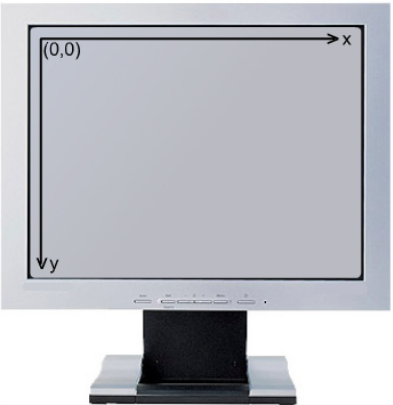
\includegraphics[width=.4\linewidth]{coord}
  \caption{Axis disposition}
\end{minipage}%
	\begin{minipage}{.5\textwidth}
  \centering
  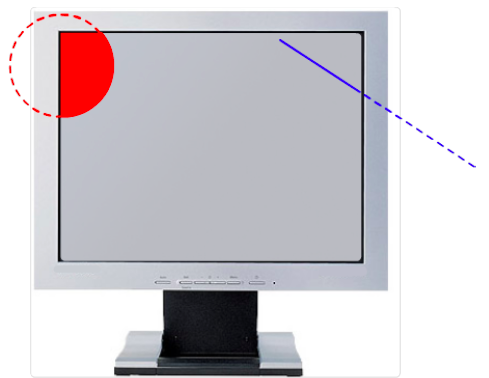
\includegraphics[width=.55\linewidth]{clipping}
  \caption{clipping}
\end{minipage}%
\end{figure}

\subsection{Point primitives}
The \textbf{point} is the simplest 2D primitive which consists in setting a \textbf{pixel} in given \textbf{position \& color}.\\
Generally the graphic primitive that draws the point is called \texttt{plot()} but the \textbf{actual} way in which a point is drawn is \textbf{hardware dependent} : every adapter has its own plot() algorithm.\\
\newpage
\subsubsection{Linear Interpolation}
A very simple numerical way to compute \textbf{intermediate points} giving \textbf{two} known points is called \textbf{interpolation} : $$I(x_0,x,x_1,y_0,y_1) = y = y_0+(x-x_0)\frac{y_1-y_0}{x_1-x_0} $$ where $ (x_0,y_0) , (x_1,y_1) $ are the known values.\\
Interpolation can be used to find N-1 intermediate points, equally spaced among two points $ (x_0,y_0), (x_N,y_N) $ :  $$I(0,i,N,y_0,y_N) = y_i = y_0+\frac{y_N-y_0}{N}i $$. \\Alternatively $y_i$ can be found \textbf{recursively} starting from $y_{i-1}$ : 
$$ y_i = y_0+\frac{y_N-y_0}{N}i \text{ where } dy= \frac{y_N-y_0}{N} \to y_1 = y_{i-1} + dy $$
\newpage
\subsection{Line primitives}
The \textbf{line primitives} connect \textbf{two points} $(x_0,y_0) , (x_1,y_1) $ on screen with a straight segment. Each pixel that composes the line (except for $ p_0 , p_1 $ must touch another pixel to keep the line continuous. The \textbf{number of pixels} involved depends on the \textbf{angle} between the line and the x-axis : 
$$ N = max(|x_1-x_0|,|y_1-y_0|)+1 $$ which corresponds to 
\[ \text{Number of pixels} =
\begin{cases}
	\theta < 45° & \quad |x_1-x_0|+1 \\
	\theta > 45° & \quad |y_1-y_0|+1 
\end{cases}
\]\\
\begin{figure}[H]
 \centering
  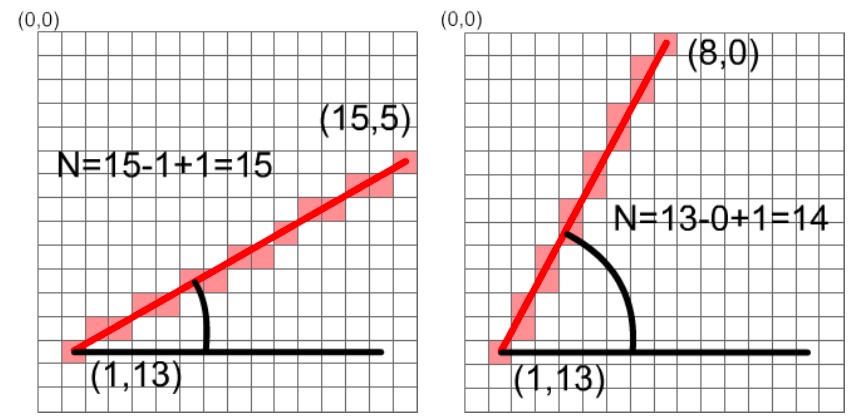
\includegraphics[width=.7\linewidth]{pixelnum}
\end{figure}
After finding the number of required pixels, different algorithms perform the line drawing task. Two main algorithms are :
\begin{itemize}
\item Interpolation algorithm : floating points operations (good on modern hardware)
\item Bresenham algorithm : integer operations (good on old or embedded/ special purpose hardware)
\end{itemize}
\newpage
\subsubsection{Interpolation Algorithm}
A popular line drawing algorithm is the Interpolation algorithm.

\begin{lstlisting}
{
   if( |x1-x0| >= |y1-y0|){ //Angle >45 o <45?
   	if(x0 > x1){			   // to get smallest value as index in for loop
   		swap(x0,y0,x1,y1); 
   	}
   	y=y0;
   	dy = (y1-y0)/(x1-x0); //interpolation increment (can be negative!!)
   	for(x=x0;x<=x1;x++){
   		plot(x,round(y),c); //rounding to nearest int
   		y += dy;
   	}
   }else{
   	  	if(y0 > y1){
   		swap(x0,y0,x1,y1);
   	}
   	x=x0;
   	dx = (x1-x0)/(y1-y0);
   	for(y=y0;y<=y1;y++){
   		plot(round(x),y,c);
   		x += dx;
   	}
}
\end{lstlisting}
\newpage
\subsubsection{Bresenham Algorithm}
The algorithm has 8 different implements depending on which \textbf{octant} the points lie : 
\begin{figure}[H]
 \centering
  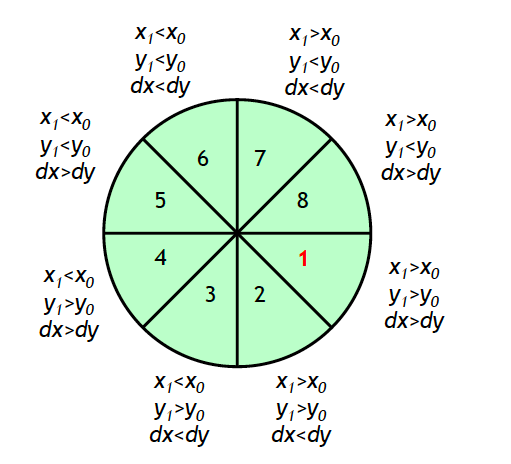
\includegraphics[width=.4\linewidth]{octants}
\end{figure}
Using octant 1 a example :
\begin{enumerate}
\item Step. : Find the number of pixels $ N = max{|x_1-x_0|,|y_1-y_0|}+1$
\item Step. : First pixel drawn in its position
\item Step. : Depending on the slope select the feasible pixels
\begin{figure}[H]
 \centering
  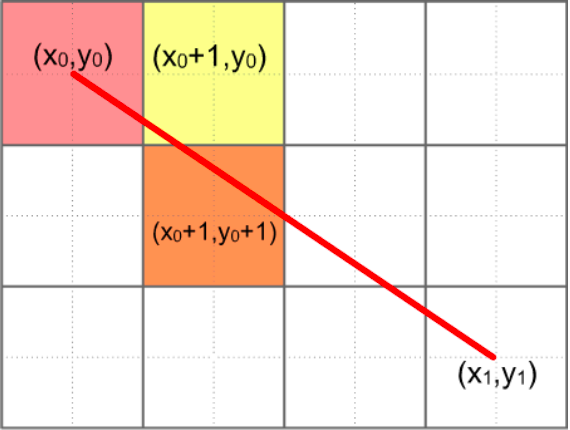
\includegraphics[width=.3\linewidth]{pixelsel}
\end{figure}
\item Step. : Select the pixels whose center is closer to the line ( orange pixel )
\item Step. : The process is repeated from step 2 until the end is reached. At each iteration y (in this case) \textbf{remains constant} or \textbf{increases} by one depending on whether the distance from the previous pixel is greater than 0.5. If the distance is greater y is increased and the distance is reset by one.
\end{enumerate}
\begin{lstlisting}
{
	dy = (y1-y0)/(x1-x0);
	dist = 0 ;
	y=y0;
	plot(x,y,c);
	for(x=x0+1;x<=x1;x++){
		dist += dy;
		if(dist > 0.5){
			y++;
			dist = dist-1;
		}
		plot(x,y,c);
	}
}
\end{lstlisting}
The algorithm above used \textbf{floats} fro computation which is not what we wanted.
The integer version of the algorithm is obtained by \textbf{multiplying} all terms considering the distance times \textbf{2(x1-x0)}:
 
\begin{lstlisting}
{
	dy = 2(y1-y0);
	dx = x1-x0;
	idist = 0 ;
	y=y0;
	plot(x,y,c);
	for(x=x0+1;x<=x1;x++){
		idist += dy;
		if(idist > dx){
			y++;
			idist -= 2dx;
		}
		plot(x,y,c);
	}
}
\end{lstlisting}
Obviously the algorithm changes slightly for the other octants.
\begin{figure}[H]
 \centering
  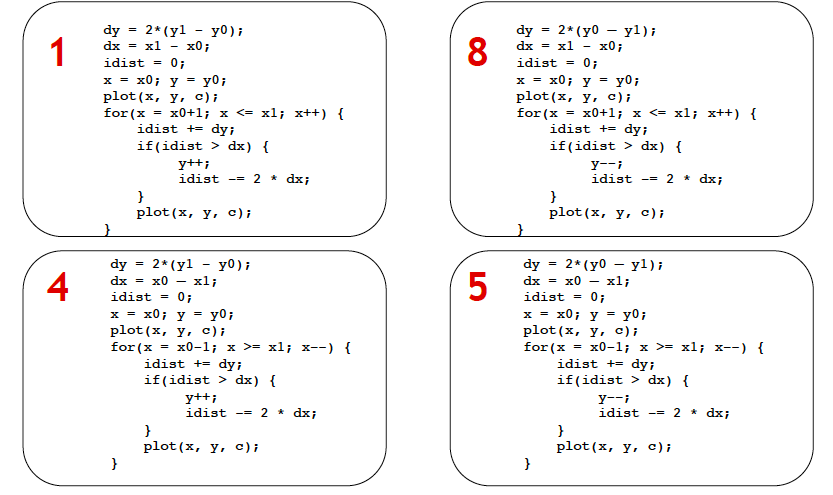
\includegraphics[width=1\linewidth]{oc2}
\end{figure}
\begin{figure}[H]
 \centering
  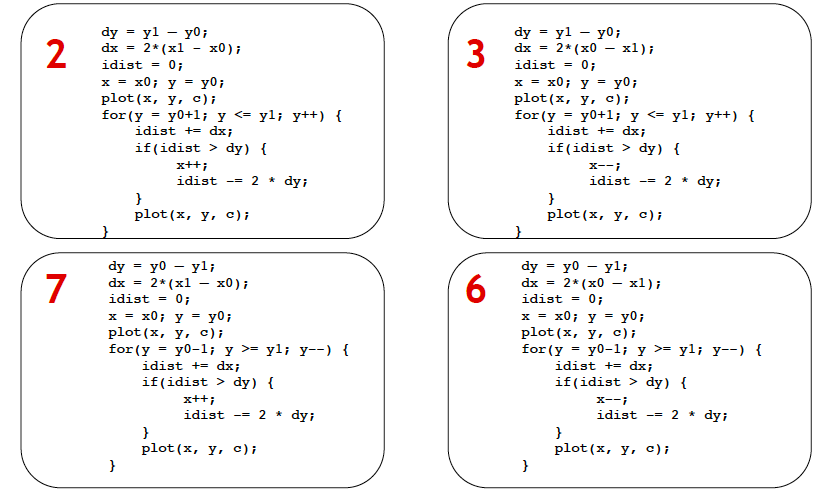
\includegraphics[width=1\linewidth]{oc1}
\end{figure}

\newpage
\subsection{Triangle Primitives}
Triangles are very important as they're the basis for \textbf{3D} computer graphics.
Triangles having one \textbf{edge parallel to the horizontal} axis is the \textbf{easiest} to draw.\\
Other triangles can be split in 2 to obtain easy to draw triangles.\\
\begin{figure}[H]
 \centering
  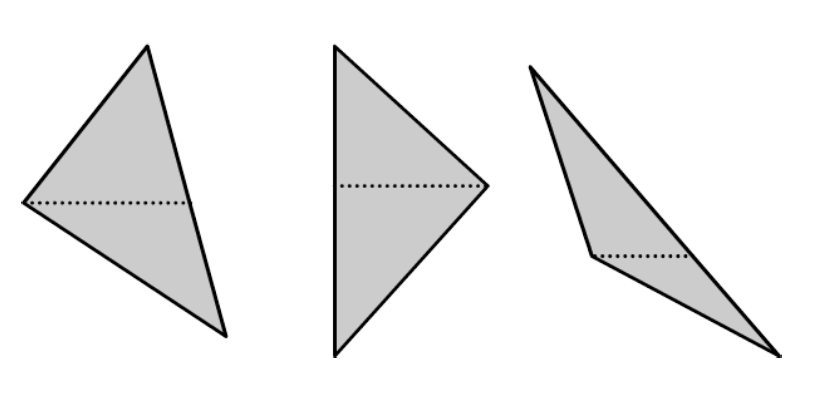
\includegraphics[width=0.5\linewidth]{tri}
\end{figure}
\subsubsection{Triangles with edge //  to x-axis}
Triangles of this type are characterized by 5 values:
\begin{itemize}
\item \textbf{$x_v$ ,$y_v$} coordinates of the vertex
\item \textbf{$y_B$} vertical coordinates of the base
\item \textbf{$x_{Bl},x_{Br}$} horizontal coordinates of the base
\end{itemize}
The two edges not parallel to x-axis can be considered as two lines.//
The triangles is \textbf{filled} by drawing horizontal lines that connect pixels over the angled edges.\\
The $x_l,x_r$ coordinates can be found using \textbf{interpolation}.
\begin{figure}[H]
 \centering
  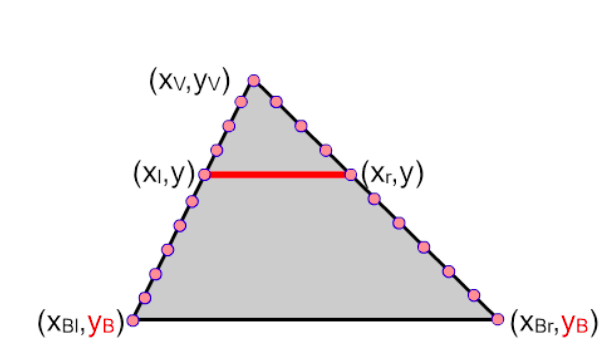
\includegraphics[width=0.5\linewidth]{tridraw}
\end{figure}

\begin{lstlisting}
{	/*since the two lines have diff. slope , store in
	dxr ,dxl the increments in the x direction */
	dxl = (xBl - xv)/(yB - yv); 
	dxr = (XBr - xv)/(yB - yv); 
	xl = xr = xv; // starting from vertex
	/* assumption yv < yB , otherwise change loop direction */
	for ( y = yv; y <=yB ; y++) {
		for(x=round(xl);x<=round(xr); x++){
			plot(x,y,c)
		}
		xl += dxl;
		xr += dxr;
	}								
}
\end{lstlisting}

\subsubsection{Triangle splitting}
More complex triangles can be split in order to obtain two triangles with edges parallel to x-axis.\\
\begin{figure}[H]
 \centering
  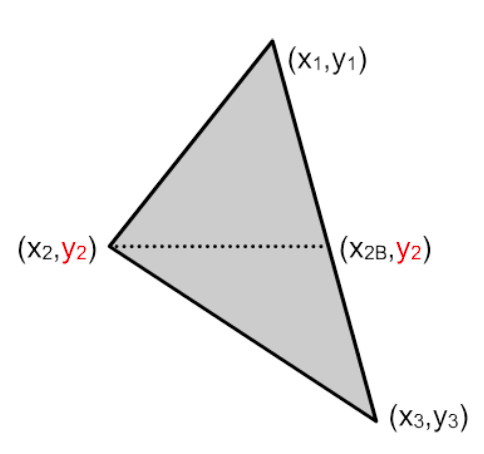
\includegraphics[width=0.3\linewidth]{trisplit}
\end{figure}
An easy way to find the middle point (x2,y2) is to take the three points and sort them through the y-axis. The one in the middle is the middle point.\\
To find the corresponding point on the opposing edge : 
\begin{itemize}
\item \textbf{y-coordinate} is the same as in point (x2,y2)
\item \textbf{x-coordinate} is obtained via \textbf{interpolation}: $$ x_{2B} = I(y_1,y_2,y_3,x_1,x_3)$$
\end{itemize}

\subsection{Normalized coordinates}
Current displays are available in different \textbf{resolutions} and \textbf{sizes}.
Moreover in windowed operating systems applications must be \textbf{confined} only in a portion of the screen.
When changing the resolutions/window size the applications still want to show the \textbf{same image} exploiting all the features of the display.
A special coordinates system called \textbf{Normalized Screen Coordinates} is normally used to address points on screen in a device in an independent way.\\
NSC are Cartesian coordinate system where x and y range between to \textbf{canonical values} [ OpenGL -1 $\to$ 1 ].  If the window/memory area resolution is known in $s_w,s_h$ pixels, the coordinates system $(x_s,y_s)$ can be derived from the normalized screen coordinates $ (x_n , y_n) $ : 
$$ x_s = (s_w-1)*(x_n+1)/2 $$ $$ y_s = (s_h-1)*(1-y_n)/2 $$ 
